\chapter{Inleiding}

Het besturingssysteem is de software-laag die de gebruiker afschermt
van de eigenlijke hardware van het computersysteem. Iets preciezer kunnen
we stellen dat het de software-laag is tussen de toepassingssoftware en de
uiteindelijke uitvoering van machine-instructies op de hardware, maar
aangezien besturingssystemen het onderwerp zijn van deze cursus ben je er
hiermee natuurlijk nog niet vanaf.

We zullen in deze cursus steeds weer twee belangrijke doelstellingen
van een besturingssysteem terugvinden. Gecompileerde toepassingssoftware
zou rechtstreeks kunnen uitgevoerd worden op de hardware, maar om het
gebruiksgemak en de effici\"entie te verhogen wordt een besturingssysteem
gebruikt.

De term "gebruiker" moet in de meest brede zin
ge\"interpreteerd worden. Het kan zowel gaan om een gewone eindgebruiker als
om een gevorderde gebruiker of een systeembeheerder. Deze verschillende
soorten gebruikers stellen andere verwachtingen aan hun computersystemen,
en het is de taak van het besturingssysteem om deze zoveel mogelijk in te
lossen.

We zullen de basisprincipes behandelen die de grondslag vormen van
het uitermate complexe gebeuren dat zich afspeelt tussen de
toepassingssoftware en de uiteindelijke uitvoering van de
machine-instructies. Een goed begrip van de verschillende controle- en
beheersfuncties die in een modern besturingssysteem zijn ingebouwd is
onmisbaar voor een informaticus. Je kan geen optimaal presterende
toepassingen ontwerpen zonder te weten hoe deze functies ge�plementeerd
worden. Ook bij het oplossen van problemen met computersystemen is het van
belang het besturingssysteem te begrijpen.

Naast algemene principes en mogelijke technieken om deze te
realiseren bestuderen we ook hoe concrete besturingssystemen
ge\"implementeerd zijn.

\section{Situering}

Voor de gebruiker van een computersysteem is de
toepassingssoftware ongetwijfeld het belangrijkste onderdeel ervan. Het
computersysteem wordt enkel gebruikt omdat het deze software kan
uitvoeren. Hierdoor kan een gebruiker er teksten mee bewerken, zijn
boekhouding bijhouden, programmeren, communiceren via een netwerk of
ingewikkelde berekeningen maken.

Nochtans is de toepassingssoftware slechts een klein onderdeel van
het volledige computersysteem, zoals wordt aangetoond in figuur \ref{situering}.

\begin{figure}
\begin{center}
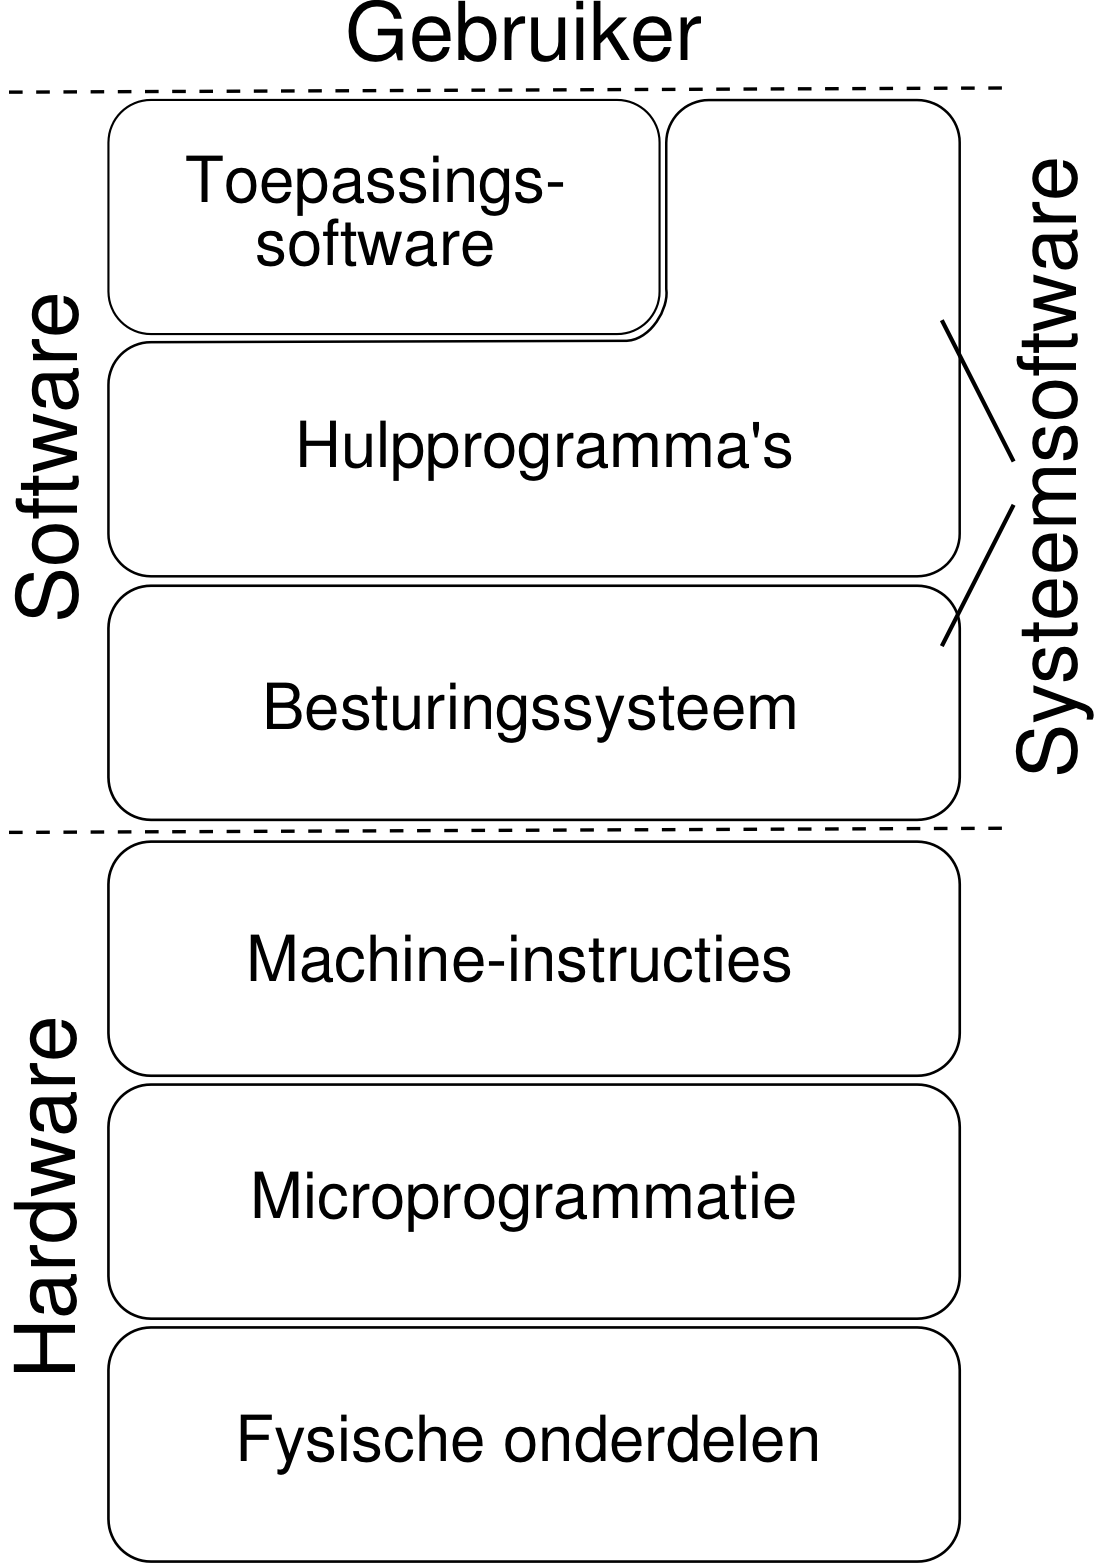
\includegraphics[width=60mm]{images/fig0101.png}
\end{center}
\caption{Situering}
\label{situering}
\end{figure}

\subsection{Hardware}

Men merkt hier een opsplitsing vooreerst in hardware en
software. De hardware zorgt voor de uitvoering van bevelen, die door
de software d.m.v. machine-instructies worden gegeven.

Deze instructies worden meestal niet rechtstreeks uitgevoerd
door de fysische onderdelen (chips, weerstanden, kabels enz.) maar via
een tussenlaag: de \emph{microprogrammatie} of
\emph{microcode}. Dit is een verzameling van kleine
programma's in machinetaal die door de processoren worden begrepen en
toelaten dat relatief ingewikkelde operaties via \'e\'en
machine-instructie kunnen worden uitgevoerd. Microcode is een
voorbeeld van wat men firmware noemt: in ROM opgeslagen software. Men
vindt firmware vaak als enige softwarelaag terug in eenvoudigere
systemen met \'e\'en specifieke taak, zoals b.v. digitale camera's,
routers of GSM's. Het is bij deze toestellen over het algemeen niet
mogelijk extra software te installeren, maar soms is het wel mogelijk
om de firmware te vervangen door een nieuwe versie. Microcode heeft
niet \'e\'en specifieke taak, maar dient om het schrijven van programma's
in machinetaal te vereenvoudigen door vaak voorkomende taken aan te
bieden in \'e\'en oproep.

\subsection{Software}

De software kan worden opgesplitst in toepassingssoftware en
systeemsoftware, die op zijn beurt bestaat uit het eigenlijke
besturingssysteem en een reeks hulpprogramma's.

Zonder de systeemsoftware is een computersysteem niet bruikbaar.
Het besturingssysteeem regelt de toegang tot de onderliggende
hardware. De hulpprogramma's worden aan het besturingssysteem
toegevoegd om het gebruik ervan te vergemakkelijken. Typische
voorbeelden zijn teksteditoren, compilers en programma's voor het
werken met bestanden.

Het uitvoeren van toepassingssoftware is het uiteindelijke doel
van het computersysteem. De enige bedoeling van de onderliggende lagen
is om dit mogelijk te maken. De hardware-lagen laten toe om
programma's in assembleertaal uit te voeren. Het besturingssysteem en
de hulpprogramma's dienen om dit zo effici\"ent en gemakkelijk mogelijk
te maken.

\section{Evolutie}

\subsection{Zonder besturingssysteem}

Bij de eerste computersystemen was nog geen sprake van een
besturingssysteem. Programma's werden in machinetaal geschreven, en de
computer kon maar 1 programma inladen en dan uitvoeren. Het laden en
starten gebeurde typisch door de programmeur zelf. Pas als een
programma afgelopen was kon het volgende geladen worden. Een programma
in uitvoering heeft in dit geval de volledige controle over alle
onderdelen van het computersysteem.

Na een tijd stelde men vast dat de geschreven programma's veel
gelijkaardige routines bevatten, b.v. voor in- en uitvoer. Ieder
programma moet gegevens inlezen, en moet op de een of andere manier
resultaten uitvoeren. Om te vermijden dat iedere programmeur deze
stukken machinecode opnieuw moest schrijven begonnen fabrikanten van
computersystemen \emph{bibliotheken} met vaak
gebruikte routines bij hun produkten te leveren. Een programmeur kon
zijn programma dan linken met code uit deze bibliotheken. Dit
vereenvoudigt het programmeren, maar de machine kan nog steeds maar
\'e\'en programma tegelijkertijd uitvoeren, en dit programma krijgt de
volledige controle over het systeem.

Bij het gebruik van de hierboven beschreven computersystemen
traden meer en meer planningsproblemen op. Er moest een planning
opgesteld worden om te bepalen wie de computer wanneer mocht
gebruiken. Als een programma vroeger dan voorzien klaar was, stond het
systeem stil tot de programmeur die het volgende tijdblok gereserveerd
had aankwam. Dat zo'n duur systeem tijdens dergelijke 'idle time'
ongebruikt blijft wilde men natuurlijk zo veel mogelijk vermijden.
Wanneer een programma langer moet rekenen dan voorzien ontstaat er ook
een probleem. Ofwel moet de volgende in de planning wachten, ofwel
moet het programma afgebroken worden en moet er nieuwe tijd
ingeroosterd worden. Bovendien bestaat de kans dat een programma door
een programmeerfout vastloopt. Het computersysteem wordt dan ook niet
gebruikt terwijl de programmeur de fout opspoort. Als de tijd op is
moet de programmeur opnieuw tijd inroosteren om het nog eens te
proberen.\footnote{Op dergelijke systemen was er nog geen sprake van
interactieve debuggers. Je kon je programma ook niet vlug even
aanpassen en opnieuw testen. Een programma moest bij iedere
wijziging opnieuw op ponskaarten gezet, ingeladen en uitgevoerd
worden. Er wordt wel eens gezegd dat de hedendaagse
informatica-studenten slechtere of alleszins minder zorgvuldige
programmeurs zouden zijn door het toegenomen
gebruiksgemak...}

\subsection{Een mens als besturingssysteem!?}

Om de planningsproblemen te ondervangen werd na verloop van tijd
een \emph{menselijke operator} ge\"introduceerd.
Programmeurs brengen de uit te voeren programma's naar de operator, op
ponskaarten, papierband of magneetband. Het laden en starten van de
verschillende programma's is nu de taak van de operator. Hierdoor zijn
de problemen met de planning grotendeeels opgelost. De operator
bezorgt de programmeur het resultaat van zijn programma, of eventueel
de inhoud van het geheugen op het moment dat er een fout optrad. Met
deze zogenaamde \emph{core dump}\footnote{De term core dump is
afgeleid van magnetic core memory, \'e\'en van de eerste types computergeheugen.
Zie
b.v. \url{http://en.wikipedia.org/wiki/Core_memory}}
kan de programmeur dan op zoek naar de fout.

Er ontstaan ook extra mogelijkheden doordat de programma's
aangeleverd worden, en dan door de operator gestart worden. Er kunnen
prioriteiten toegekend worden aan verschillende programma's. De
operator kan hiermee rekening houden bij het bepalen van de volgorde
waarin de programma's gestart worden. Hij moet niet noodzakelijk de
volgorde waarin ze aangeleverd worden respecteren. De operator kan ook
gegevens bijhouden, b.v. de gebruikte computertijd per programma. Met
deze gegevens kan het gebruik van het computersysteem eventueel
gefactureerd worden aan de gebruikers. Later werden meer gegevens
genoteerd, zoals het aantal geprinte pagina's, ingelezen ponskaarten,
operator-interventies, hoeveelheid gebruikte schijfruimte, ...

Computersystemen worden steeds sneller, maar de menselijke
operatoren niet. Hierdoor worden zij meer en meer de vertragende
factor. Als een operator 10 seconden nodig heeft om een programma te
starten, en het programma duurt 90 seconden, dan gaat er 10 \% van de
tijd naar de operator. Als de computer 3 keer sneller wordt, is het
programma voltooid na 30 seconden. De totale tijd wordt 40 seconden,
en het aandeel van de operator is al goed voor 25 \%.

Bovendien laten de krachtigere systemen, waarvan ook de
opslagcapaciteit blijft toenemen, toe dat de door de fabrikant
meegeleverde bibliotheken alsmaar meer en complexere taken vervullen.
Zo kunnen ze de facturatiegegevens bijhouden, en het volgende
programma starten. Zo wordt de vertraging van de menselijke operator
gedeeltelijk weggewerkt. Als de bibliotheken ook nog proberen te
voorkomen dat er misbruik gemaakt wordt van de beschikbare
hulpmiddelen van het systeem, kunnen we stellen dat ze evolueren naar
de eerste besturingssystemen.

\subsection{De eerste besturingssystemen}

We kunnen eigenlijk pas van een besturingssysteem spreken vanaf
het moment dat de zogenaamde \emph{residente monitors}
gebruikt worden, omdat zo'n residente monitor instaat voor de controle
van het systeem, \'en constant in het geheugen gehouden worden (vandaar
'resident').

De residente monitor wordt gedurende de ganse werkperiode van de
computer in het geheugen gehouden en zorgt ervoor dat een uit te
voeren programma in het geheugen wordt geladen en gestart. Daartoe
wordt een sprong uitgevoerd naar het beginadres van het programma, en
wordt aan het einde van het programma een sprong naar de monitor
toegevoegd. Zo kan de monitor het computersysteem voortdurend
controleren, eventueel in samenspraak met de operator. De operator
moet wel nog steeds zorgen voor het aanbieden van de uit te voeren
programma's, maar de rest van het beheer is overgenomen door de
residente monitor.

Uit de codebibliotheken die bij de computersystemen geleverd
worden evolueren ook specifieke besturingsroutines voor randapparaten,
\emph{device drivers} genoemd. Door deze drivers wordt
het geven van opdrachten aan en het communiceren met randapparatuur
eenvoudig. Een programma moet gewoon de juiste functie van de driver
aanroepen. Wanneer je programma gebruik moest maken van een ander type
randapparaat, moest je nu enkel nog de oproep van de device driver
aanpassen. Samen met de opkomst van de hogere programmeertalen zorgden
de device drivers dat het voor veel meer ge\"interesseerden mogelijk
werd om computers te gebruiken.

Deze eerste besturingssystemen groeien uit tot eenvoudige
\emph{batch-besturingssysteem}. De term batch (groep,
verzameling) wijst op de gebruikswijze van dit soort systemen: men
biedt een stel programma's als een globaal pakket aan het
besturingssysteem aan en deze programma's worden dan onder controle
van dit systeem en zonder verdere tussenkomst van een gebruiker of
operator \'e\'en na \'e\'en uitgevoerd.

\subsection{Multiprogrammatie en Time Sharing}

Batch-besturingssystemen kennen een steeds groter wordend
effici\"entie-probleem. Terwijl het programma dat ze aan het uitvoeren
zijn wacht op het voltooien van in- of uitvoer, wordt de processor van
het computersysteem niet gebruikt. Bovendien nam het belang van deze
perioden van inactiviteit toe naarmate de processoren sneller
werden.

Als oplossing worden de besturingssystemen uitgebreid met
\emph{multiprogrammatie}. Terwijl een programma moet
wachten op een externe gebeurtenis laat het besturingssysteem de
processor verderwerken aan een ander programma. Dit leidt tot een
situatie waarin een reeks verschillende programma's samen in het
geheugen aanwezig zijn en om de beurt worden uitgevoerd tot ze moeten
wachten. Het lijkt dan alsof de computer al deze programma's tegelijk
uitvoert, maar de processor is altijd maar met \'e\'en van de programma's
bezig.

Wanneer een multiprogrammatie-systeem wordt uitgebreid met een
\emph{spooling}-systeem (SPOOL: Simultaneous
Peripheral Operation OnLine), dat een aantal jobs kan klaarhouden op
een snel extern geheugen en de simultane\footnote{Zoals gezegd is deze simultane
uitvoer slechts schijn, de computer werkt eigenlijk om de beurt aan de
verschillende programma's, maar het probleem is wel re\"eel. Als deze
programma's b.v. regelmatig een lijn naar een printer sturen is het natuurlijk
niet de bedoeling dat de uitvoer naar de printer van beide programma's op
\'e\'en blad vermengd wordt.} uitvoer (output) van verschillende jobs op een
ordelijke manier kan afhandelen komt men tot een zeer krachtig
besturingssysteem.

De multiprogrammatie-systemen kenden nog een groot gebrek: het
gebrek aan interactiviteit. Het is nog steeds zo dat men een programma
laat uitvoeren en dan wacht op het resultaat. Als dat resultaat niet
is wat men verwachtte, moet men het programma wijzigen en opnieuw
laten uitvoeren. De schijnbaar simultane uitvoer van programma's bij
multiprogrammatie laat ook toe om verschillende gebruikers tegelijk op
een interactieve wijze met een computer te laten werken. Elke
gebruiker beschikt dan over een in- en uitvoerapparaat, verbonden met
de centrale verwerkingseenheid, dat hem toelaat met de computer te
communiceren. Omdat de processor afwisselend gedurende korte tijd aan
elke gebruiker wordt toegewezen krijgt elk van hen de indruk
voortdurend te beschikken over alle faciliteiten van het
computersysteem. Deze vorm van multiprogrammatie wordt \emph{time
sharing} genoemd. Het belangrijkste verschil met de
hierboven beschreven multiprogrammatie is dat er bij time sharing niet
gewacht wordt tot een programma moet wachten om de processor aan een
ander programma toe te kennen.

Doordat de gebruiker op een time sharing systeem rechtstreeks
met de computer kan communiceren, krijgt hij bijna onmiddellijk
feedback bij kleinere opdrachten. Hierdoor neemt het gebruikscomfort
sterk toe. Doordat gebruikers typisch niet tegelijkertijd pieken
veroorzaken in het processorgebruik lijkt het systeem voor ieder van
hen toch performant te werken. Je zou kunnen zeggen dat de computer de
invoer meestal sneller kan verwerken dan de gebruiker ze kan
genereren. Hierdoor kan de computer meerdere gebruikers tegelijk
bedienen. Voor het accepteren van invoer via een toetsenbord moet de
processor zeer weinig werk verrichten, dus terwijl de ene gebruiker
een opdracht typt, is er processorkracht over voor het inlezen van de
toetsenborden van andere gebruikers, of het werken aan eerder gegeven
opdrachten. Als er dan nog processorkracht over is, kan eventueel nog
steeds aan niet-interactieve batch-verwerking van opdrachten gedaan
worden. Als er veel interactief gebruik is moeten de batch-taken
wachten.

\subsection{Besturingssystemen voor Minicomputers}

In de jaren 60 kwamen de \emph{minicomputers} op
de markt. Laat je niet misleiden, zo'n minicomputer was 'mini' omdat
hij maar enkele kasten in beslag nam terwijl de eerdere systemen een
volledige kamer in beslag namen. Tot dan had men gewoon van computers
gesproken, maar nu werden de grotere modellen mainframes genoemd. Men
zegt ook soms dat de minicomputers de eerste computers waren die door
\'e\'en persoon bediend konden worden.

Bij mainframes was het de gewoonte dat een fabrikant een
besturingssysteem ontwikkelde telkens hij een nieuw model op de markt
bracht. Dit was voor de fabrikant een zware inspanning, maar voor de
gebruiker betekende het ook telkens grote conversieproblemen als er
naar een nieuwere en krachtigere computer overgeschakeld werd. Al de
programma's moesten namelijk aangepast worden aan het nieuwe
besturingssysteem.

In 1964 lanceerde IBM voor het eerst een familie van
computersystemen. De System/360 reeks van mainframes omvatte modellen
met verschillende verwerkingscapaciteiten, maar ze waren allemaal
gebaseerd op dezelfde architectuur. Dit liet toe op al deze modellen
hetzelfde besturingssysteem te gebruiken en betekende dat bij het
overgaan naar een ander model van dezelfde reeks bijna alle
conversieproblemen verdwenen. Alle modellen gebruikten dan ook (een
variant van) hetzelfde besturingssysteem: OS/360. Omdat OS/360 voor
allerlei soorten toepassingen moest gebruikt worden, werd het een zeer
ingewikkeld besturingssysteem. Deze systemen werden soms
multimode-systemen genoemd omdat ze zoveel verschillende werkwijzen
moesten aankunnen.

Door de opkomst van de minicomputers groeide de markt voor
computersystemen. Door deze stijging van het aantal computergebruikers
ging er meer aandacht naar de gebruiksvriendelijkheid en de
interactiviteit van de besturingssystemen. De PDP's (Programmed Data
Processor) van Digital Equipment waren een zeer succesvolle reeks van
minicomputers. De PDP-1 kwam op de markt in 1961. Voor
\$120.000\footnote{Dit zijn "1960 dollars", wat zou overeenkomen
met meer dan 700.000 hedendaagse dollars. Dit lijkt veel, maar voor een gewone
mainframe betaalde je in 1960 al gauw \$1.000.000 (ook "1960 dollars")} had je
een machine met een geheugencapaciteit van 4000 woorden van 18 bits, m.a.w. 9
kilobyte. Een andere vroege minicomputer was de LINC, ook van DEC. Figuur \ref{linc_specs} toont de specificaties van de LINC uit de oorspronkelijke brocure uit 1961. Figuur \ref{linc_prijs} toont een prijslijst.

\begin{figure}
\begin{center}
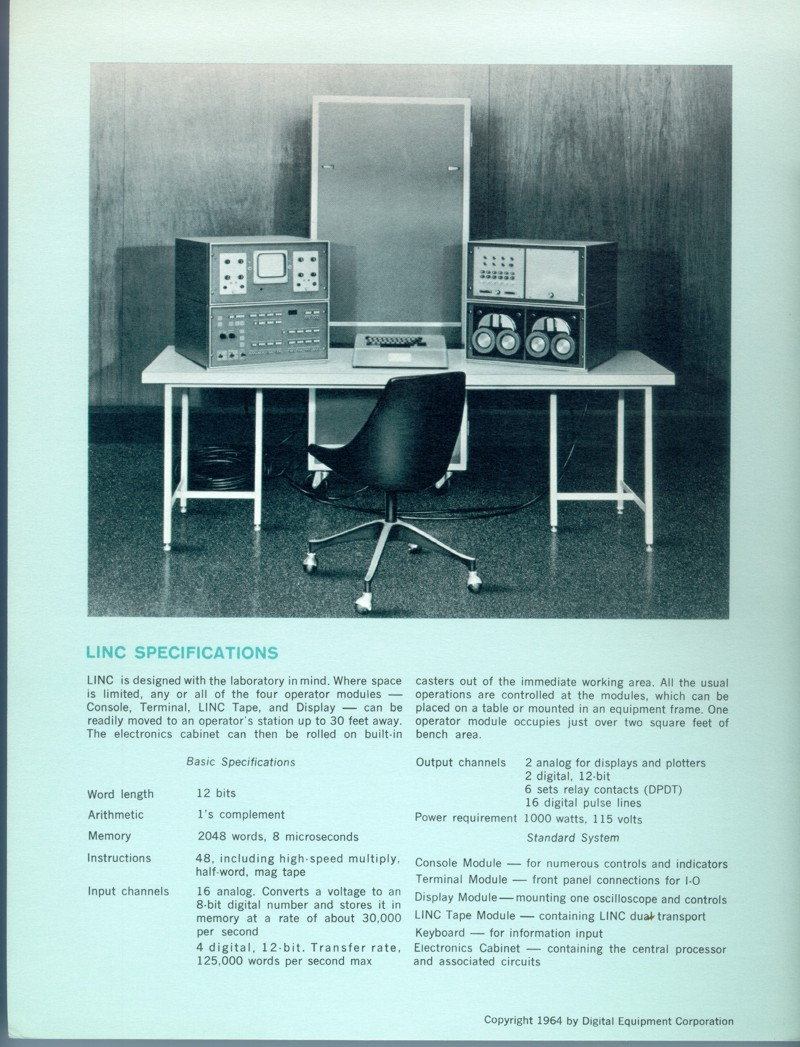
\includegraphics[width=\textwidth]{images/linc01.jpg}
\end{center}
\caption{LINC Specificaties}
\label{linc_specs}
\end{figure}

\begin{figure}
\begin{center}
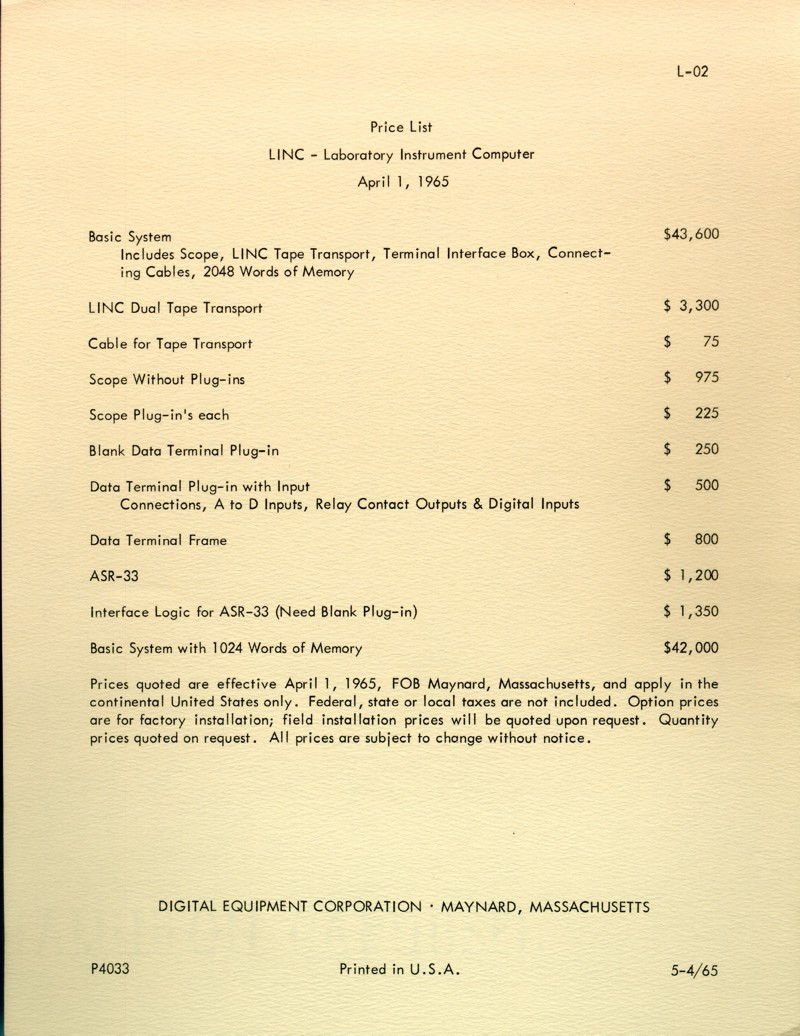
\includegraphics[width=\textwidth]{images/linc02.jpg}
\end{center}
\caption{LINC Prijslijst}
\label{linc_prijs}
\end{figure}

In de wetenschappelijke wereld raakte intussen stilaan
\emph{UNIX} bekend, een nieuw besturingssysteem dat
niet door een computerconstructeur werd ontwikkeld en waar (althans
oorspronkelijk) geen commerci\"ele bedoelingen aan vastzaten. Het was
een klein besturingssysteem met multiprogrammatie en ondersteuning
voor meerdere gebruikers. De belangrijkste nieuwigheid was dat het,
mits enkele kleine aanpassingen, op elke hardware bruikbaar kon worden
gemaakt en daarbij naar de gebruiker toe steeds dezelfde interface
bood. Dit was ondermeer te danken aan het feit dat het niet in een
assembleertaal, maar in een daarvoor speciaal ontwikkelde hogere
programmeertaal, C genaamd, was geschreven. De ontwikkeling van UNIX
wekte voor het eerst de hoop op een standaard-besturingssysteem en
probleemloos uitwisselbare toepassingssoftware.

\subsection{De PC en het Internet}

Wat men van UNIX verwachtte werd in de jaren 80 vrij onverwacht
gerealiseerd, zij het op een totaal andere manier. Aand het eind van
de jaren 70 dook de microcomputer op. Toen IBM zijn
\emph{microcomputer}, de Personal Computer of PC,
lanceerde en hiervoor een nieuw besturingssysteem, MS-DOS, liet
ontwikkelen bleek dit zo'n groot succes dat de meeste andere
constructeurs deze architectuur overnamen. Hierdoor ontstond een
enorme markt met uniforme computers: de IBM-compatibele PC's. Men kon
nu toepassingssoftware ontwikkelen die op zowat 90\% van de zich
massaal verspreidende microcomputers kon worden gebruikt.

De grote verspreiding van de microcomputer zorgde ervoor dat
eigenlijk iedereen met een computer wou gaan werken. Hierdoor moest er
dringend werk gemaakt worden van een vereenvoudiging van de
gebruikersinterface. Vandaar de ontwikkeling van GUI's (Graphical User
Interfaces), waarmee op een symbolische manier bevelen aan de computer
konden worden gegeven. In 1984 kwam de Apple Macintosh SE op de markt,
de eerste computer met een GUI. De SE kostte \$2495, en bevatte een 8
MHz processor en een werkgeheugen van 4 MB. In 1985 was er dan de
eerste versie van Windows, een grafische laag bovenop MS-DOS. Een GUI
is een mooi voorbeeld van een hulpprogramma dat bij het eigenlijke
besturingssysteem zit om het gebruik ervan te vereenvoudigen.

De stijgende performantie van de microcomputer was ideaal voor
multitasking: time sharing voor \'e\'en gebruiker. De gebruiker kan
verschillende opdrachten tegelijk laten uitvoeren, en deze opdrachten
laten samenwerken. De processortijd wordt door het besturingssysteem
verdeeld over al de opdrachten.

De gebrekkige communicatie tussen computers was het volgende
obstakel. Dit leidde tot het introduceren van netwerken. Eerst LANs,
daarna WANs en uiteindelijk de wereldwijde verbindingen tussen al deze
netwerken. Het geheel kennen we nu als het Internet.

\section{Voorbeelden van Besturingssystemen}

Bij het bespreken van de evolutie van besturingssystemen kwamen al
enkele voorbeelden aan bod zoals OS/360 en MS-DOS. Aangezien
besturingssystemen sinds OS/360 niet meer specifiek voor \'e\'en bepaalde
machine ontworpen worden, zijn ze nu meestal verbonden met \'e\'en van de
drie besproken types: mainframes, minicomputers of
microcomputers.

Doordat iedereen nu over een PC beschikt lijkt het misschien alsof
mainframes afgedaan hebben, maar dat blijkt niet het geval. IBM is nog
steeds \'e\'en van de grote spelers in de mainframe-markt, en er worden nog
steeds mainframes ontwikkeld. De S/360 reeks is ge\"evolueerd naar de
S/370 en later de S/390 reeks. Nu worden de IBM mainframes zSeries
genoemd. De besturingssystemen die in de loop der jaren voor deze
systemen ontwikkeld zijn omvatten klinkende namen als MVS, VM en
VSE.

Ook minicomputers zijn nog steeds te verkrijgen en in gebruik. Men
spreekt nu ook soms van midrange systemen, en IBM noemt ze iSeries. In
de jaren 80 waren er twee grote concurrenten in dit segment. Digital
(later Compaq en nu HP) had de VAX-machines, met als besturingssysteem
VMS, en OS/400 op de IBM AS/400 computers.

Voor microcomputers waren er in de jaren 80 drie families. Op
IBM-compatibele PC's had je de keuze tussen MS-DOS van Microsoft en OS/2
van IBM. Voor Macintosh computers was er System 7. OS/2 is van de markt
verdwenen, en MS-DOS is ge\"evolueerd naar de verschillende versies van
Windows. Windows was eerst slechts een grafische toevoeging aan MS-DOS,
maar de recentere versies zijn volledige besturingssystemen. Voor
Macintosh computers heb je tegenwoordig MacOS nodig.

Er zijn ook besturingssystemen die niet aan \'e\'en van de 3 grote
categorie\"en van computersystemen verbonden zijn. Ze kunnen in principe
op iedere computer worden gebruikt. Allereerst is er UNIX dat men op de
meest diverse hardware aantreft, zij het in allerlei varianten. Op
mainframes vind je AIX (IBM) als gast onder VM. Op VAX minicomputers
werd Ultrix (later Digital Unix) gebruikt terwijl voor microcomputers
SCO Unix (vroeger Xenix) of HPUX beschikbaar is. Voor PC's (maar ook
voor andere platformen) is er sinds 1991 ook het steeds populairdere
GNU/Linux.

In deze cursus zullen we vooral Windows en Linux als voorbeeld
gebruiken.

\section{Functies van een besturingssysteem}

Zoals reeds aangehaald heeft het besturingssysteem twee grote
taken: het \emph{gebruiksgemak} en de
\emph{effici\"entie} van het computersysteem maximaliseren.
Naar de gebruiker toe proberen we b.v.:

\begin{description}
\item[De toegang tot apparaten eenvoudig te maken]Toepassingssoftware moet b.v.
op een eenvoudige manier in- en uitvoerapparaten kunnen aanspreken. Device
drivers laten toe abstractie te maken van de specifieke hardware.
\item[Informatie bewaren en overzichtelijk weergeven]Gebruikers willen hun
gegevens opslaan en later terug ophalen. Het besturingssysteem moet opslagmedia
zoals harde schijven bruikbaar maken.
\item[Operaties en gegevens beveiligen]Gegevens van verschillende gebruikers of
programma's moeten afgeschermd worden van andere gebruikers of programma's.
\end{description}

Wat betreft de hardware wordt er getracht:

\begin{description}
\item[De onderlinge communicatie tussen onderdelen te organiseren]
\item[De goede werking van de onderdelen bewaken]Wanneer er een fout optreedt in
de hardware moet die gedetecteerd en zo mogelijk gecorrigeerd worden.
\item[Hulpmiddelen rechtvaardig te verdelen]Verschillende gebruikers en
programma's willen gebruik maken van de aanwezige hulpmiddelen, en het
besturingssysteem staat in voor de verdeling.
\end{description}

Merk op dat het besturingssysteem ook een programma is dat door de
processor uitgevoerd moet worden. De gebruiker van een systeem wil
alleen zijn software uitvoeren, en niet het besturingssysteem. We kunnen
dus stellen dat de tijd dat het besturingssysteem de processor gebruikt
verloren gaat voor de gebruiker. Effici\"entie is dus een belangrijke
vereiste voor het besturingssysteem, om de hoeveelheid overhead te
beperken. Het is belangrijk te beseffen dat, hoewel het in theorie om
onnuttige processortijd gaat, het besturingssysteem ervoor zou moeten
zorgen dat de computer beter gebruikt wordt. Enerzijds wordt de computer
gemakkelijker om te gebruiken, en anderzijds ontstaan er mogelijkheden
die er zonder besturingssysteem niet zouden zijn, zoals het uitvoeren
van meerdere programma's tegelijkertijd.

Een derde taak voor het besturingssysteem is om te streven naar
\emph{hardware-onafhankelijkheid}. Als het
besturingssysteem een uniforme interface aanbiedt aan de de
bovenliggende toepassingssoftware en de gebruiker kan de hardware
aangepast worden zonder overgangsproblemen, zoals ge\"illustreerd in 
figuur \ref{platform}. In de bespreking van de evolutie van 
besturingssystemen zijn we hiervan al enkele voorbeelden tegengekomen.
De eerste stap naar hardware-onafhankelijkheid was de introductie 
van device drivers.

\begin{figure}
\begin{center}
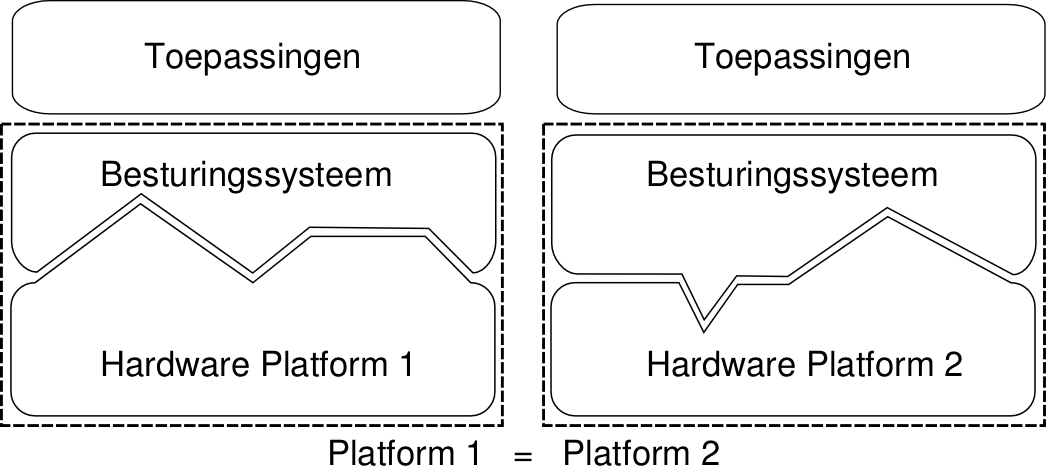
\includegraphics[width=80mm]{images/fig0102.png}
\end{center}
\caption{Besturingssysteem zorgt voor hardware-onafhankelijkheid}
\label{platform}
\end{figure}

Er zijn versies van de Linux-kernel voor verschillende
architecturen, b.v. x86, Alpha, SPARC, ARM en S/390. Toepassingssoftware
die geschreven is voor de Linux-kernel kan dus op ieder van deze
architecturen uitgevoerd worden.

\section{Onderdelen van een besturingssysteem}

Om de werking van een besturingssysteem te begrijpen moeten we
verschillende onderdelen bestuderen. Onderstaande componenten komen
ieder in meer detail aan bod verder in deze cursus.

\subsection{Bestandsbeheer}

Op opslagmedia zoals b.v. magneetschijven kunnen enen en nullen
weggeschreven worden. Omdat dit niet handig is bieden de meeste
besturingssystemen de gebruiker de mogelijkheid om met bestanden te
werken. Het besturingssysteem zal deze bestanden dan op opslaan op de
schijf en ze terug inlezen wanneer de gebruiker daarom vraagt.
Bovendien zal ook rekening gehouden moeten worden met aspecten zoals
toegangscontrole en optimaal gebruik van beschikbare
schijfruimte.

\subsection{Apparaatbeheer}

De toegang tot de randapparatuur moet door het besturingssysteem
geregeld worden, om b.v. conflicten te vermijden. Als 2 programma's
tegelijkertijd naar de printer zouden kunnen schrijven zouden we
vreemde resultaten krijgen.

\subsection{Geheugenbeheer}

Computerprogramma's kunnen niet uitgevoerd worden zonder toegang
tot werkgeheugen, maar ook hier komt enige organisatie aan te pas.
Programma's mogen b.v. niet in elkaars geheugensegmenten lezen of
schrijven. Aangezien het beschikbare werkgeheugen beperkt is moet het
besturingssysteem ook streven naar effici\"ent gebruik ervan.

\subsection{Procesbeheer}

Procesbeheer omvat in essentie het verdelen van de beschikbare
processortijd over de verschillende processen die uitgevoerd moeten
worden. Hier wordt gezorgd voor multiprogrammatie en
multitasking.

\subsection{Communicatie}

Het besturingssysteem staat in voor de communicatie tussen
processen op het computersysteem, maar ook voor eventuele communicatie
met andere computersystemen via een netwerk.

\subsection{Gebruikersinterface}

Om het gebruik van de computer te vereenvoudigen moet het
besturingssysteem ook zorgen voor een adequate gebruikersinterface.
Dit kan een tekstgebaseerde interface aan een commandoprompt zijn,
maar ook een grafische omgeving is mogelijk. Deze taak hangt samen met
al de andere, omdat de gebruiker natuurlijk een interface nodig heeft
om het bestandssysteem aan te spreken.

